\documentclass[a4paper]{article}

\def\nbook {All of Statistics: A Concise Course in Statistical Inference}
\def\nbookshort {All of Statistics}

% Shared preamble. The fallback lets the document build whether the working
% directory is its own folder or the project root.
\IfFileExists{headerallofstats.tex}{\input{headerallofstats}}{%%%%%%%%%%%%%%%%%%%%
% AUTHOR AND HEADER
% define \nbook
%%%%%%%%%%%%%%%%%%%%

\makeatletter
\ifx \nauthor\undefined
  \def\nauthor{David A. Lee}
\else
\fi

\author{\nbook \\ \small Solutions by \nauthor}
\date{}

%%%%%%%%%%%%%%%%%%%%
% PACKAGES
%%%%%%%%%%%%%%%%%%%%

\usepackage{alltt} 
\usepackage{amsfonts}
\usepackage{amsmath}
\usepackage{amssymb}
\usepackage{amsthm}
\usepackage{bm}
\usepackage{booktabs}
\usepackage{caption}
\usepackage{centernot}
\usepackage{enumitem}
\usepackage{fancyhdr}
\usepackage[T1]{fontenc}
\usepackage{graphicx}
% Images live in chap1/ ... chap8/ at the project root, while the documents that
% use them sit one level down (allofstats/, allofstatschap1/, ...). Listing both
% "./" and "../" lets a document keep writing \includegraphics{chap1/foo.eps}
% and still resolve it whether it is compiled from its own folder or from the
% project root.
\graphicspath{{./}{../}}
\usepackage{mathdots}
\usepackage{mathtools}
\usepackage{microtype}
\usepackage{multirow}
\usepackage{pdflscape}
\usepackage{pgfplots}
\pgfplotsset{compat=1.18}
\usepackage{siunitx}
\usepackage{slashed}
\usepackage{tabularx}
\usepackage{tikz}
\usepackage{titletoc}
\usepackage{tkz-euclide}
\usepackage[normalem]{ulem}
\usepackage{url}
\usepackage[all]{xy}
\usepackage{imakeidx}

% fonts
% use \textsf to change to Computer Modern Bright
\renewcommand{\sfdefault}{cmbr} % keeps default font Computer Modern Roman

% makeindex for table of contents
\makeindex[intoc, title=Index]
\indexsetup{othercode={\lhead{ Index }}}

% table of contents remove numbering
\setcounter{secnumdepth}{0}

% pagestyle
\pagestyle{fancyplain}

% header
\lhead{	\nouppercase{\leftmark} }
\ifx \nextra \undefined
  \rhead{
    \ifnum\thepage=1
    \else
      \nbookshort \  | \nauthor
    \fi}
\else
  \rhead{
    \ifnum\thepage=1
    \else
      \nbookshort (\nextra)
    \fi}
\fi

% proof environment

\newcommand{\prooffont}{\scshape}
\usepackage{xpatch}
\tracingpatches
\xpatchcmd{\proof}{\itshape}{\prooffont}{}{}

% Python environment (for typesetting Python code)

% Default fixed font does not support bold face
\DeclareFixedFont{\ttb}{T1}{txtt}{bx}{n}{8} % for bold
\DeclareFixedFont{\ttm}{T1}{txtt}{m}{n}{8}  % for normal

% Custom colors
\usepackage{color}
\definecolor{deepblue}{rgb}{0,0,0.5}
\definecolor{deepred}{rgb}{0.6,0,0}
\definecolor{deepgreen}{rgb}{0,0.5,0}

\usepackage{listings}

% Python style for highlighting
\newcommand\pythonstyle{\lstset{
language=Python,
basicstyle=\ttm,
morekeywords={self},              % Add keywords here
keywordstyle=\ttb\color{deepblue},
emph={MyClass,__init__},          % Custom highlighting
emphstyle=\ttb\color{deepred},    % Custom highlighting style
stringstyle=\color{deepgreen},
frame=tb,                         % Any extra options here
showstringspaces=false
}}


% Python environment
\lstnewenvironment{python}[1][]
{
\pythonstyle
\lstset{#1}
}
{}

% Python for external files
\newcommand\pythonexternal[2][]{{
\pythonstyle
\lstinputlisting[#1]{#2}}}

% Python for inline
\newcommand\pythoninline[1]{{\pythonstyle\lstinline!#1!}}

%%%%%%%%%%%%%
% FUNCTIONS %
%%%%%%%%%%%%%

\DeclarePairedDelimiter\abs{\lvert}{\rvert}%
\DeclarePairedDelimiter\norm{\lVert}{\rVert}%

%%%%%%%%%%%%%%%%%%%%
% DOCUMENT GEOMETRY
%%%%%%%%%%%%%%%%%%%%

\ifx \ntrim \undefined
\else
  \usepackage{geometry}
  \geometry{
	  papersize={379pt, 699pt},
	  textwidth=345pt,
	  left=17pt,
	  top=54pt,
	  right=17pt,
  }
\fi

% maketitle statement
\title{}
\ifx \nisofficial \undefined
\let\@real@maketitle\maketitle
\renewcommand{\maketitle}{\@real@maketitle\begin{center}\begin{minipage}[c]{0.9\textwidth}\centering\footnotesize All errors, typographical and substantive, and other offenses, are entirely my own.\end{minipage}\end{center}}
\else
\fi

%%%%%%%%%%%%%%%%%%%%
% THEOREMS
%%%%%%%%%%%%%%%%%%%%

%\theoremstyle{definition}
\newtheorem*{axiom}{Axiom}
\newtheorem*{claim}{Claim}
\newtheorem*{conjecture}{Conjecture}
\newtheorem*{cor}{Corollary}
%\newtheorem*{dfn}{Definition}
\newtheorem*{eg}{Example}
\newtheorem*{ex}{Exercise}
%\newtheorem*{lemma}{Lemma}
\newtheorem*{prop}{Proposition}
%\newtheorem*{thm}{Theorem}
\newtheorem*{remark}{Remark}
\newtheorem*{warning}{Warning}

%%%%%%%%%%%%%%%%%%%%
% FORMATTING AESTHETICS
%%%%%%%%%%%%%%%%%%%%

% itemize bullets
\renewcommand{\labelitemi}{-}
\renewcommand{\labelitemii}{$\circ$}
\renewcommand{\labelenumi}{(\roman{*})}

% new page section
\let\stdsection\section
\renewcommand\section{\newpage\stdsection}

%%%%%%%%%%%%%%%%%%%%
% \mathbb commands
%%%%%%%%%%%%%%%%%%%%

\newcommand{\C}{\mathbb{C}}
\newcommand{\N}{\mathbb{N}}
\newcommand{\Q}{\mathbb{Q}}
\newcommand{\R}{\mathbb{R}}
\newcommand{\Z}{\mathbb{Z}}


%%%%%%%%%%%%%%%%%%%%
% Probability Operators
%%%%%%%%%%%%%%%%%%%%

\DeclareMathOperator{\Bernoulli}{Bernoulli}
\DeclareMathOperator{\betaD}{Beta}
\DeclareMathOperator{\bias}{\textsf{bias}}
\DeclareMathOperator{\binomial}{Binomial}
\DeclareMathOperator{\corr}{Corr}
\DeclareMathOperator{\cov}{\textsf{Cov}}
\DeclareMathOperator{\Exp}{Exp}
\DeclareMathOperator{\gammaD}{Gamma}
\DeclareMathOperator{\mse}{\textsf{MSE}}
\DeclareMathOperator{\multinomial}{Multinomial}
\DeclareMathOperator{\Poisson}{Poisson}
\DeclareMathOperator{\sd}{sd}
\DeclareMathOperator{\se}{\textsf{se}}
\DeclareMathOperator{\Uniform}{Uniform}
\newcommand{\Prob}{\mathbb{P}}
\newcommand{\var}{\mathbb{V}}
\newcommand{\E}{\mathbb{E}}

%%%%%%%%%%%%%%%%%%%%
% TCOLORBOX CODE FROM SeniorMars
%%%%%%%%%%%%%%%%%%%%

%\usepackage[varbb]{newpxmath} changes math font to newpxmath
\usepackage{xfrac}
\usepackage[makeroom]{cancel}
\usepackage{mathtools}
\usepackage{bookmark}
\usepackage{enumitem}
\usepackage{hyperref,theoremref}
\hypersetup{
	pdftitle={Assignment},
	colorlinks=true, linkcolor=doc!90,
	bookmarksnumbered=true,
	bookmarksopen=true
}
\usepackage[most,many,breakable]{tcolorbox}
\usepackage{xcolor}
\usepackage{varwidth}
\usepackage{varwidth}
\usepackage{etoolbox}
%\usepackage{authblk}
\usepackage{nameref}
\usepackage{multicol,array}
\usepackage{tikz-cd}
\usepackage[ruled,vlined,linesnumbered]{algorithm2e}
\usepackage{comment} % enables the use of multi-line comments (\ifx \fi)
\usepackage{import}
\usepackage{xifthen}
\usepackage{pdfpages}
\usepackage{transparent}

\newcommand\mycommfont[1]{\footnotesize\ttfamily\textcolor{blue}{#1}}
\SetCommentSty{mycommfont}
\newcommand{\incfig}[1]{%
    \def\svgwidth{\columnwidth}
    \import{./figures/}{#1.pdf_tex}
}

\usepackage{tikzsymbols}

% colors -- change them as you may!

\definecolor{myg}{RGB}{56, 140, 70}
\definecolor{myb}{RGB}{45, 111, 177}
\definecolor{myr}{RGB}{199, 68, 64}
\definecolor{mytheorembg}{HTML}{F2F2F9}
\definecolor{mytheoremfr}{HTML}{00007B}
\definecolor{mylenmabg}{HTML}{FFFAF8}
\definecolor{mylenmafr}{HTML}{983b0f}
\definecolor{mypropbg}{HTML}{f2fbfc}
\definecolor{mypropfr}{HTML}{191971}
\definecolor{myexamplebg}{HTML}{F2FBF8}
\definecolor{myexamplefr}{HTML}{88D6D1}
\definecolor{myexampleti}{HTML}{2A7F7F}
\definecolor{mydefinitbg}{HTML}{E5E5FF}
\definecolor{mydefinitfr}{HTML}{3F3FA3}
\definecolor{notesgreen}{RGB}{0,162,0}
\definecolor{myp}{RGB}{197, 92, 212}
\definecolor{mygr}{HTML}{880808}
\definecolor{myred}{RGB}{127,0,0}
\definecolor{myyellow}{RGB}{169,121,69}
\definecolor{myexercisebg}{HTML}{F2FBF8}
\definecolor{myexercisefg}{HTML}{88D6D1}
\definecolor{doc}{RGB}{0,60,110}

%================================
% THEOREM BOX
%================================

%\providecommand\theoremnumber{}
\tcbuselibrary{theorems,skins,hooks}
\newtcbtheorem{Theorem}{Theorem}
{%
	enhanced,
	breakable,
	colback = mytheorembg,
	frame hidden,
	boxrule = 0sp,
	borderline west = {2pt}{0pt}{mytheoremfr},
	sharp corners,
	detach title,
	before upper = \tcbtitle\par\smallskip,
	coltitle = mytheoremfr,
	fonttitle = \bfseries\sffamily,
	description font = \mdseries,
	separator sign none,
	segmentation style={solid, mytheoremfr},
}
{th}


%================================
% Question BOX
%================================

\makeatletter
\newtcbtheorem{question}{Question}{enhanced,
	breakable,
	colback=white,
	colframe=mygr,
	attach boxed title to top left={yshift*=-\tcboxedtitleheight},
	fonttitle=\bfseries\sffamily,
	title={#2},
	boxed title size=title,
	boxed title style={%
			sharp corners,
			rounded corners=northwest,
			colback=tcbcolframe,
			boxrule=0pt,
		},
	underlay boxed title={%
			\path[fill=tcbcolframe] (title.south west)--(title.south east)
			to[out=0, in=180] ([xshift=5mm]title.east)--
			(title.center-|frame.east)
			[rounded corners=\kvtcb@arc] |-
			(frame.north) -| cycle;
		},
	#1
}{def}
\makeatother

%================================
% PROPERTIES BOX
%================================

\tcbuselibrary{theorems,skins,hooks}
\newtcbtheorem{Property}{Property}
{%
	enhanced,
	breakable,
	colback = mytheorembg,
	frame hidden,
	boxrule = 0sp,
	borderline west = {2pt}{0pt}{mytheoremfr},
	sharp corners,
	detach title,
	before upper = \tcbtitle\par\smallskip,
	coltitle = mytheoremfr,
	fonttitle = \bfseries\sffamily,
	description font = \mdseries,
	separator sign none,
	segmentation style={solid, mytheoremfr},
}
{th}

%================================
% LEMMA
%================================

\tcbuselibrary{theorems,skins,hooks}
\newtcbtheorem[number within=section]{Lemma}{Lemma}
{%
	enhanced,
	breakable,
	colback = mylenmabg,
	frame hidden,
	boxrule = 0sp,
	borderline west = {2pt}{0pt}{mylenmafr},
	sharp corners,
	detach title,
	before upper = \tcbtitle\par\smallskip,
	coltitle = mylenmafr,
	fonttitle = \bfseries\sffamily,
	description font = \mdseries,
	separator sign none,
	segmentation style={solid, mylenmafr},
}
{th}


% Commands for special boxes
\newcommand{\thm}[2]{\begin{Theorem*}{#1}{}#2\end{Theorem*}}
\newcommand{\qs}[2]{\begin{question*}{#1}{}#2\end{question*}}
\newcommand{\prp}[2]{\begin{Property*}{#1}{}#2\end{Property*}}
\newcommand{\lemma}[2]{\begin{Lemma*}{#1}{}#2\end{Lemma*}}
}

\begin{document}
\maketitle

\section{Chapter 3: Expectation}

\subsection*{Import Packages}

Please see the associated GitHub repo for all code and comments to simulations. [LINK HERE]

% QUESTION 1
\qs{3.8.1}{Suppose we play a game where we start with \(c\) dollars. On each play of the game you either double or halve your money, with equal probability. What is your expected fortune after \(n\) trials?}

By premise, \(\Prob(X = 2c) = 1/2, \Prob(X = \frac{1}{2}c) = 1/2\). By definition of expectation, we have
\[
	\E(X) = 2c \left( \frac{1}{2} \right) + \frac{1}{2}c \left( \frac{1}{2} \right) = \boxed{\frac{5}{4}c} 
\]

Simulating the money game, we find:

\begin{center}
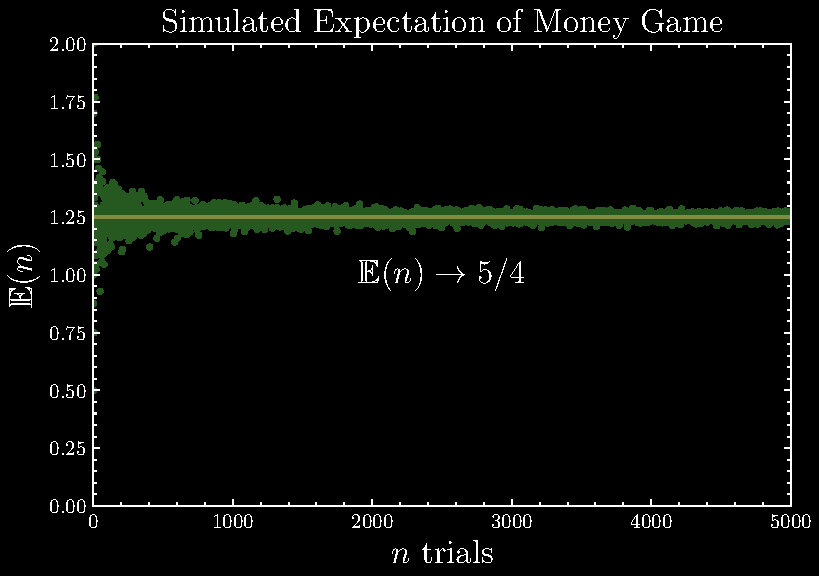
\includegraphics[width=1.0\textwidth]{chap3/chap3ex1.eps}
\end{center}

% QUESTION 2
\qs{3.8.2}{Show that \(\var(X) = 0 \) if and only if there is a constant \(c\) such that \(\Prob(X = c) = 1\).}
\begin{proof}[Proof] 
\(( \implies )\) Let \(\var(X) = 0\). Since \(\var(X) = \int (x - \mu)^{2}  \ dF(x) \), we must have \(x = \mu\). Then \(\Prob(X = \mu) = 1\).\vspace{12pt}
\par \((\impliedby)\) Let \(\Prob(X = c) = 1\). Then \(\E(X) = c\) and \(\E(X^{2}) = c^{2}\). Then \(\var(X) = \E(X^{2}) - \E(X)^{2} = c^{2} - c^{2} = 0\).
\end{proof}

% QUESTION 3
\qs{3.8.3}{Let \(X_{1},\dots,X_{n} \sim \Uniform(0,1)\) and let \(Y_{n} = \max\{X_{1},\dots,X_{n}\}\). Find \(\E(Y_{n})\).}

Assume \textsf{IID} standard uniform variables. Note that \(Y_{n} \le y\) if and only if \(X_{1},\dots,X_{n} \le y\). We can derive
\begin{align*}
	F_{Y_{n}}(y) & = \Prob(Y_{n} \le y) \\
	 & = \prod_{i=1}^{n} \Prob(X_{i} \le y)  \\
	 & = \prod_{i=1}^{n} \int^{y}_{0}  \ dx_{i} \\
	 & = y^{n}
\end{align*}
Then the \textsf{PDF} is
\[
	F_{Y_{n}}'(y) = f_{Y_{n}}(y) = ny^{n-1}
\]
and the expectation is
\[
	\E(Y_{n}) = \int^{1}_{0} ny^{n} \ dy = \boxed{\frac{n}{n+1}} 
\]

% QUESTION 4
\qs{3.8.4}{A particle starts at the origin of the real line and moves along the line in jumps of one unit. For each jump the probability is \(p\) that the particle will jump one unit to the left and the probability is \(1-p\) that the particle will jump one unit to the right. Let \(X_{n}\) be the position of the particle after \(n\) units. Find \(\E(X_{n})\) and \(\var(X_{n})\). (This is known as a \textbf{random walk}.)}

We define \(X\) as
\[
	X = \begin{cases}
		+1 & 1 - p \\
		-1 & p \\
	\end{cases}
\]
After one jump, 
\begin{align*}
	\E(X_{i}) & = 1(1-p) + (-1)p = 1 - 2p \\
	\E(X_{i}^{2}) & = 1 - p + p = 1 \\ 
	\var(X_{i}) & = \E(X_{i}^{2}) - \E(X_{i})^{2} = 1 - (1-2p)^{2} = 4(p - p^{2})
\end{align*}
After \(n\) jumps, assuming independence of each jump,
\begin{align*}
	\E \left( \sum_{}^{n} X_{i} \right)  & = \sum_{}^{n} \E(X_{i}) = \boxed{n(1-2p)} \\
	\var \left( \sum_{}^{n} X_{i} \right)  & = \sum_{}^{n} \var(X_{i}) = \boxed{4n(p-p^{2})} \\ 
\end{align*}

We can simulate some random walks for \(p = 0.5\):

\begin{center}
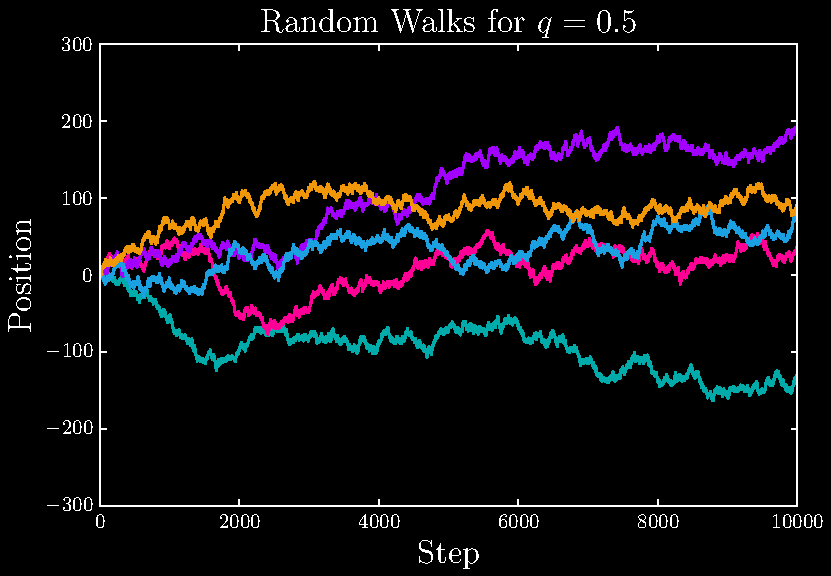
\includegraphics[width=1.0\textwidth]{chap3/chap3ex4i.eps}
\end{center}

Empirically simulating the expectation and variance for \(n\) steps also brings us quite close to our derived theoretical values:

\begin{center}
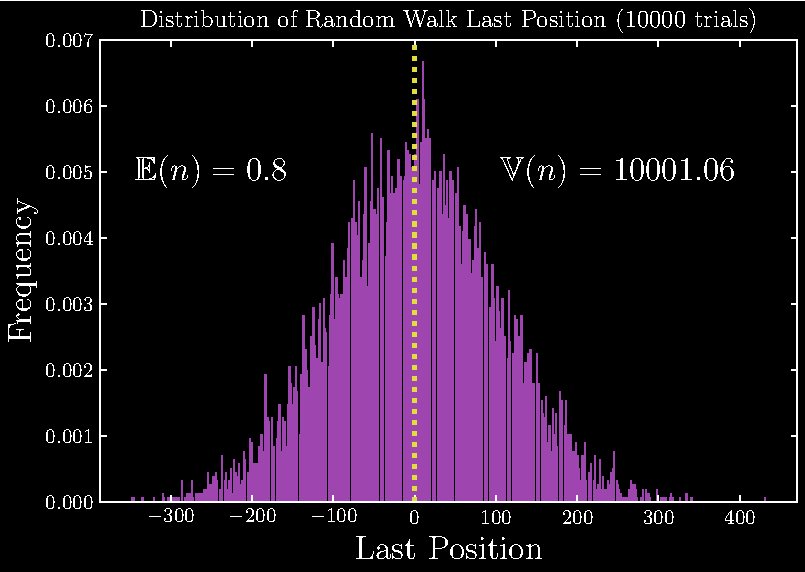
\includegraphics[width=1.0\textwidth]{chap3/chap3ex4ii.eps}
\end{center}

% QUESTION 5
\qs{3.8.5}{A fair coin is tossed until a head is obtained. What is the expected number of tosses that will be required?}

In general, for a coin in which a head is obtained with probability \(p\), we can model the expected number of tosses until we get a head with the geometric distribution:
\[
	\Prob(X = k) = p(1-p)^{k-1}
\]
Deriving the first moment, we first write the \textsf{MGF} (with \(q = 1-p)\)
\begin{align*}
	\psi_{X}(t) & \sum_{x} e^{tx}pq^{x-1} \\
	 & = p(e^{t} + qe^{2t} + q^{2}e^{3t} + \cdots ) \\ 
	 & = pe^{t}(1 + qe^{t} + q^{2}e^{2t} + \cdots ) \\
	 & = \frac{pe^{t}}{1 -qe^{t}}
\end{align*}
Differentiating gives us
\[
	\psi'_{X}(t) = pe^{t}(1-qe^{t})^{-1} - pe^{t}(-qe^{t})(1-qe^{t})^{-2}
\]
And setting \(t=0\) gives us
\begin{align*}
	\psi'_{X}(0) & p(1-q)^{-1} - p(-q)(1-q)^{-2}  \\
	 & = \frac{1}{p} 
\end{align*}
For \(p = 1/2\), \(\E(X) = \frac{1}{1/2} = \boxed{2}\). Simulating gives us the desired expectation:

\begin{center}
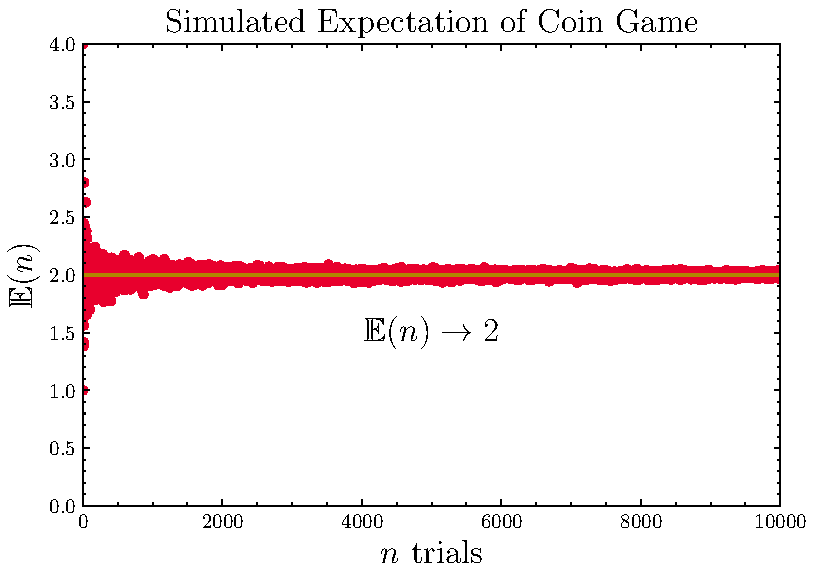
\includegraphics[width=1.0\textwidth]{chap3/chap3ex5.eps}
\end{center}

% QUESTION 6
\qs{3.8.6}{Prove Theorem 3.6 for discrete random variables.}
\begin{proof}[Proof] 
Let \(Y = r(X)\). We make no assumption about whether \(r\) is a bijection, namely if it has an inverse. Therefore, it is possible for multiple values of \(X = x\) to map to the same \(Y = y \). For instance, if \(Y = r(X) = X^{2}\), then \(X = 1\) and \(X = -1\) map to \(Y = 1\), and we have \(\Prob(Y = 1) = \Prob(X = 1) + \Prob(X = -1)\).

From the definition of expectation, we have
\[
	\E(Y) = \sum_{i} y_{i} \Prob(Y = y_{i})
\]
Now, \(\Prob(Y = y_{i})\) is equal to the sum of the probabilities of \(X\) taking on all values \(x_{j}\) such that \(y_{i} = g(X = x_{j})\). In other words,
\[
	\Prob(Y = y_{i}) = \sum_{j:y_{i}= g(x_{j})} \Prob(X = x_{j}) = \Prob(X = x)
\]
Thus we can conclude with
\begin{align*}
	 & = \sum_{i} y_{i} \sum_{j: y_{i} = g(x_{j})} \Prob(X = x_{j}) \\
	 & = \sum g(x)\Prob(X = x) \\
	 & = \sum g(x) f_{X}(x)
\end{align*}
\end{proof}

% QUESTION 7
\qs{3.8.7}{Let \(X\) be a continuous random variable with \textsf{CDF} \(F\). Suppose that \(\Prob(X > 0) = 1\) and that \(\E(X)\) exists. Show that \(\E(X) = \int^{\infty}_{0} \Prob(X > x) \ dx \).

Hint: Consider integrating by parts. The following fact is helpful: if \(\E(X)\) exists then \(\lim_{x \to \infty} x[1 - F(x)] = 0.\)}
\begin{proof}[Proof] 
By definition of expectation for a continuous random variable,
\[
	\E(X) = \int^{\infty}_{0} x f_{X}(x) \ dx 
\]
Proceeding with integration by parts, let \(\mu = x, dv = f_{X}(x) dx\). Then \(du = dx, v = F_{X}(x)\). We continue with
\begin{align*}
	 & = x F_{X}(x) \bigg| ^{\infty}_{0} - \int^{\infty}_{0} F_{X}(x) \ dx  \\
	 & = x \bigg| ^{\infty}_{0} - \int^{\infty}_{0} F_{X}(x) \ dx  \\ 
	 & = \int^{\infty}_{0}  \ dx - \int^{\infty}_{0} F_{X}(x) \ dx \\  
	 & = \int^{\infty}_{0} [1 - F_{X}(x)] \ dx \\
	 & = \int^{\infty}_{0} \Prob(X > x) \ dx 
\end{align*}
with the second equality following from the fact that \(\lim_{x \to \infty} x[1 - F_{X}(x)] = 0\), implying that \(\lim_{x \to \infty} x = \lim_{x \to \infty} x F_{X}(x) \). 
\end{proof}

\newpage
% QUESTION 8
\qs{3.8.8}{Prove Theorem 3.17.}
\thm{(Wasserman 3.17)}{Let \(X_{1},\dots,X_{n}\) be \textsf{IID} and let \(\mu = \E(X_{i}), \sigma^{2} = \var(X_{i}) \). Then
\[
	\E(\overline{X}_{n}) = \mu, \quad \var(\overline{X}_{n}) = \frac{\sigma^{2}}{n} \quad \text{and} \quad \E(S^{2}_{n}) = \sigma^{2}.
\]}
\begin{proof}[Proof] 
Use the fact that the \(X_{i}\)'s are \textsf{IID}.
\begin{align*}
	\E(\overline{X}_{n}) & = \E \left( \frac{1}{n} \sum_{i=}^{n} X_{i} \right)  \\
	 & = \frac{1}{n} \E \left( \sum_{i=1}^{n} X_{i} \right)  \\ 
	 & = \frac{1}{n} \sum_{i=1}^{n} \E(X_{i}) \\
	 & = \frac{1}{n} (n \mu) \\
	 & = \boxed{\mu} \\
	\var(\overline{X}_{n}) & = \var \left( \frac{1}{n} \sum_{i=1}^{n} X_{i} \right) \\
	 & = \sum_{i=1}^{n} \frac{1}{n^{2}} \var(X_{i}) \\
	 & = \frac{1}{n^{2}} (n \sigma^{2}) \\
	 & = \boxed{\frac{\sigma^{2}}{n}} 
\end{align*}
\begin{align*}
	\E(S^{2}_{n}) & = \E \left( \frac{1}{n-1} \sum_{i=1}^{n} (X_{i} - \overline{X}_{n})^{2} \right)  \\
	 & = \E \left( \frac{1}{n-1} \sum_{i=1}^{n} (X_{i}^{2} - 2X_{i}\overline{X}_{n} + \overline{X}_{n}^{2}) \right)  \\ 
	 & = \E \left( \frac{1}{n-1} \sum_{i=1}^{n} X_{i}^{2} - n \overline{X}_{n}^{2} \right) \\
	 & = \frac{1}{n-1} \left( \sum_{i=1}^{n} \E(X_{i}^{2}) - n \E(\overline{X}_{n}^{2}) \right) \\
	 & = \frac{1}{n-1}(n(\sigma^{2} + \mu^{2})) - \frac{1}{n-1}\frac{1}{n}(n(n-1) \mu^{2} + n(\sigma^{2} + \mu^{2})) \\
	 & = \frac{1}{n-1}(n(\sigma^{2} + \mu^{2})) - \frac{1}{n-1}(n \mu^{2} + \sigma^{2}) \\
	 & = \frac{n \sigma^{2} - \sigma^{2}}{n-1} \\
	 & = \boxed{\sigma^{2}}
\end{align*}
\end{proof}

% QUESTION 9
\qs{3.8.9}{\textsf{(Computer Experiment.)} Let \(X_{1}, X_{2}, \dots, X_{n}\) be \(N(0,1)\) random variables and let \(\overline{X}_{n} = n^{-1} \sum_{i=1}^{n} X_{i}\). Plot \(\overline{X}_{n}\) versus \(n\) for \(n = 1, \dots, 10,000\). Repeat for \(X_{1}, X_{2},\dots, X_{n} \sim \) Cauchy. Explain why there is such a difference.}

We can code our functions to generate \(\overline{X}_{n}\) for the \(N(0,1)\) and Cauchy distributions as follows:

The simulations yield:

\begin{center}
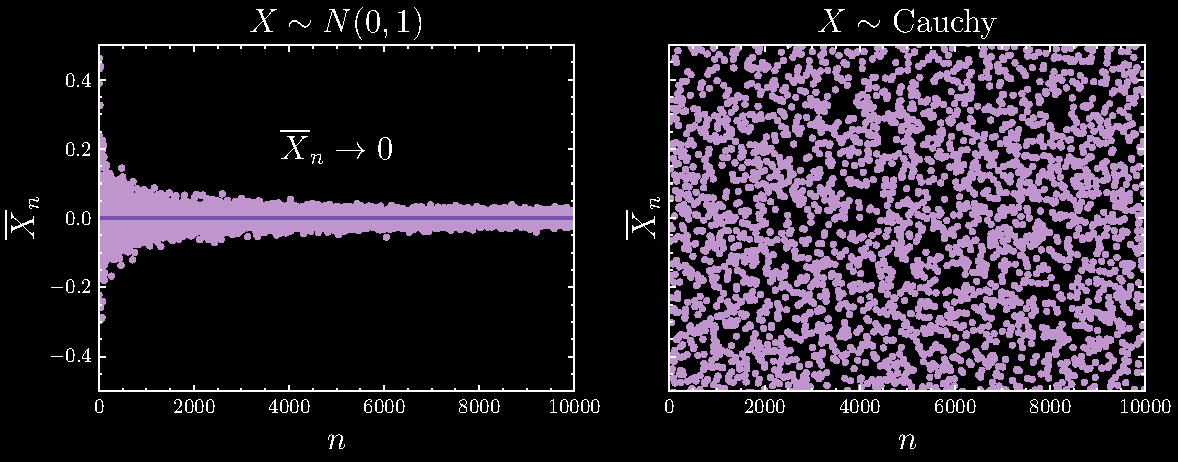
\includegraphics[width=1.0\textwidth]{chap3/chap3ex9.eps}
\end{center}

A striking comparison! Qualitatively, the standard normal and standard Cauchy distributions look to be quite similar. But notably, the latter \textit{has no mean}. Given the \textsf{PDF}
\[
	f_{Z}\left( z \right) = \frac{1}{\pi (1 + z^{2})}, \quad z \in \mathbb{R}
\]
which is generated by finding the distribution of \(Z = X/Y\) for \(X,Y \sim N(0, \sigma^{2})\), the expectation \(\E\left( Z \right)\) turns out to diverge.

% QUESTION 10
\qs{3.8.10}{Let \(X \sim N(0,1)\) and let \(Y = e^{X}\). Find \(\E(Y)\) and \(\var(Y)\).}

By the Law of the Unconscious Statistician, we have
\begin{align*}
	\E(Y) & = \frac{1}{\sqrt{2 \pi }} \int^{\infty}_{-\infty} e^{x} e^{-x^{2}/2} \ dx  \\
	 & = \frac{1}{\sqrt{2 \pi }} \int^{\infty}_{-\infty} e^{-x^{2}/2 + x} \ dx  \\ 
\end{align*}
Using the identity
\[
	\int^{\infty}_{-\infty} e^{-ax^{2} + bx} \ dx = e^{b^{2}/4a} \sqrt{\frac{\pi }{a}}
\]
with \(a = b = 1\), we can conclude
\[
	\E(Y) = \frac{1}{\sqrt{2 \pi }} e^{1/2} \sqrt{2 \pi } = \boxed{e^{1/2}}
\]
Similarly, we calculate \(\E(Y^{2})\):
\begin{align*}
	\E(Y^{2}) & = \frac{1}{\sqrt{2 \pi }} \int^{\infty}_{-\infty} e^{2x} e^{-x^{2}/2} \ dx  \\
	 & = \frac{1}{\sqrt{2 \pi }} \int^{\infty}_{-\infty} e^{-x^{2}/2 + 2x} \ dx  \\ 
	 & = e
\end{align*}
and derive
\[
	\var(Y) = \E(Y^{2}) - \E(Y)^{2} = \boxed{e^{2} - e}
\]

Simulating, we get

\begin{center}
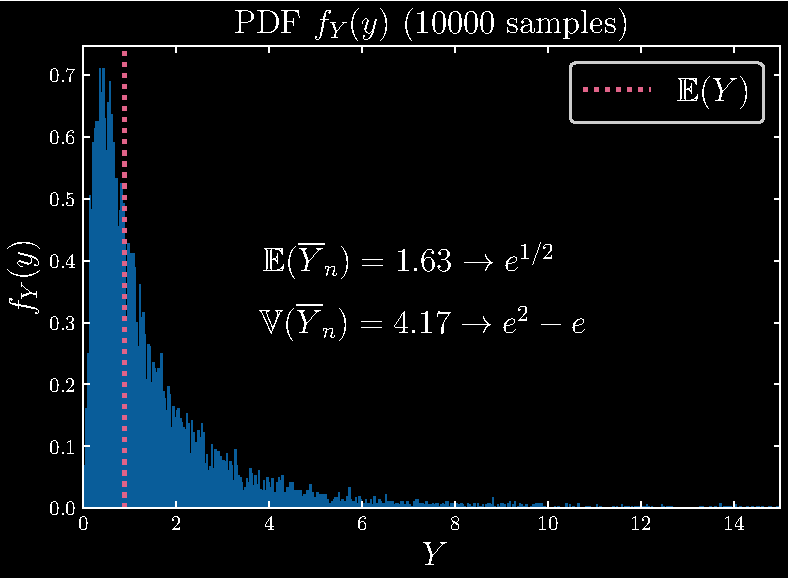
\includegraphics[width=1.0\textwidth]{chap3/chap3ex10.eps}
\end{center}

\newpage
% QUESTION 11
\qs{3.8.11}{\textsf{(Computer Experiment: Simulating the Stock Market.)} Let \(Y_{1}, Y_{2},\dots\) be independent random variables such that \(\Prob(Y_{i} = 1) = \Prob\left( Y_{i} = -1 \right) = 1/2\). Let \(X_{n} = \sum_{i=1}^{n} Y_{i}\). Think of \(Y_{i} = 1\) as "the stock price increased by one dollar," \(Y_{i} = -1\) as "the stock price decreased by one dollar," and \(X_{n}\) as the value of the stock on day \(n\).
\begin{enumerate}[label=(\alph*)]
	\item Find \(\E(X_{n})\) and \(\var(X_{n})\).
	\item Simulate \(X_{n}\) and plot \(X_{n}\) versus \(n\) for \(n = 1, 2, \dots, 10,000\). Repeat the whole simulation several times. Notice two things. First, it's easy to "see" patterns in the sequence even though it is random. Second, you will find that the four runs look very different even though they were generated the same way. How do the calculations in (a) explain the second observation?
\end{enumerate}}

(a) The expectation and variance are derived as
\begin{align*}
	\E\left( Y_{i} \right) & = 1 \cdot \frac{1}{2} - 1 \cdot \frac{1}{2} = 0\\
	\implies \E\left( X_{n} \right) & = \E\left( \sum_{i=1}^{n} Y_{i} \right) = \boxed{0} \\ 
	\E\left( Y^{2}_{i} \right) & = 1 \cdot \frac{1}{2} + 1 \cdot \frac{1}{2} = 1 \\
	\var\left( Y_{i} \right) & = \E\left( Y^{2}_{i} \right) - \E\left( Y_{i} \right)^{2} = 1 \\
	\implies \var\left( X_{n} \right) & = \var\left( \sum_{i=1}^{n} Y_{i} \right) = \boxed{n}
\end{align*}

\par (b) Refer to exercise 3.8.4, as this exercise is a special case of the random walk where \(p = 0.5\). The intuition for why the paths diverge at increasing number of steps \(n\) is because of the path-dependency of the movement of the sequence -- the position in the random walk or the stock price is contingent on what came before it -- and that the variance is dependent on \(n\) (in fact it is \(n\) itself). For high \(n\), the larger the spread of \(X_{n}\). 

\newpage
% QUESTION 12
\qs{3.8.12}{Prove the formulas given in the table at the beginning of Section 3.4 for the Bernoulli, Poisson, Uniform, Exponential, Gamma, and Beta. Here are some hints. For the mean of the Poisson, use the fact that \(e^{a} = \sum_{x=0}^{\infty} a^{x}/x!\). To compute the variance, first compute \(\E(X(X-1))\). For the mean of the Gamma, it will help to multiply and divide by \(\Gamma(\alpha + 1)/\beta^{\alpha +1}\) and use the fact that a Gamma density integrates to 1. For the Beta, multiply and divide by \(\Gamma(\alpha + 1) \Gamma(\beta) / \Gamma(\alpha + \beta + 1)\).}
\begin{proof}[Proof] 
\underline{Bernoulli}
\begin{align*}
	\E(X) & = 1 \cdot \Prob(X = 1) + 0 \cdot \Prob(X = 0) = \boxed{p} \\
	\E(X^{2}) & = 1^{2} \cdot \Prob(X = 1) + 0^{2} \cdot \Prob(X = 0) = p \\ 
	\var(X) & = \E(X^{2}) - \E(X)^{2} = p - p^{2} = \boxed{p(1-p)}
\end{align*}

\underline{Poisson}
Using the infinite sum definition of \(e^{x}\):
\[
	e^{x} = \sum_{k=1}^{\infty} \frac{x^{k-1}}{(k-1)!}
\]
we can derive
\begin{align*}
	\E(X) & = \sum_{x=0}^{\infty} xe^{-\lambda } \frac{\lambda^{x}}{x!} \\
	 & = \sum_{x=1}^{\infty} e^{-\lambda } \frac{\lambda^{x}}{(x-1)!} \\ 
	 & = \lambda e^{-\lambda } \sum_{x=1}^{\infty} \frac{\lambda^{x-1}}{(x-1)!} \\
	 & = \lambda e^{-\lambda }e^{\lambda } \\
	 & = \boxed{\lambda } \\
	\E(X(X-1)) & = \sum_{x=0}^{\infty} x(x-1) e^{-\lambda } \frac{\lambda^{x}}{x!} \\
	 & = \lambda \sum_{x=1}^{\infty} (x-1) e^{-\lambda } \frac{\lambda^{x-1}}{(x-1)!} \\
	 & = \lambda^{2}
\end{align*}
which implies \(\E(X^{2}) = \lambda^{2} + \lambda \), and in turn
\[
	\var(X) = \E(X^{2}) - \E(X)^{2} = \lambda^{2} + \lambda - \lambda^{2} = \boxed{\lambda }
\]

\underline{Uniform}
\begin{align*}
	\E(X) & = \int^{b}_{a} x \left( \frac{1}{b-a} \right)  \ dx  \\
	      & = \boxed{\frac{a + b}{2}} \\
	\E(X^{2}) & = \int^{b}_{a} x^{2} \left( \frac{1}{b-a} \right)  \ dx \\
	      & = \frac{a^{2} + ab + b^{2}}{3} \\
	\var(X) & = \E(X^{2}) - \E(X)^{2} \\
	      & = \frac{a^{2} + ab+ b^{2}}{3} - \left( \frac{a+b}{2} \right)^{2} \\
	      & = \boxed{\frac{(b-a)^{2}}{12}}
\end{align*}

\underline{Exponential}
We will have to carry out this integration by parts. Let \(\mu = x, dv = \exp(-x/\beta ) dx\). Then \(du = dx, v = -\beta \exp(-x/\beta )\).
\begin{align*}
	\E(X) & = \frac{1}{\beta } \int^{\infty}_{0} x \exp(-x/\beta ) \ dx  \\
	 & = \frac{1}{\beta } \left( -\beta x \exp(-x/\beta ) \bigg|^{\infty}_{0} + \int^{\infty}_{0} \beta \exp(-x/\beta ) \ dx  \right)   \\
	 & = -\beta \exp(-x/\beta ) \bigg| ^{\infty}_{0} \\
	 & = \boxed{\beta }
\end{align*}
To calculate \(\E(X^{2})\), let \(\mu = x, dv = x \exp(-x/\beta ) dx\), then \(du = dx, v = -(\beta x + \beta^{2}) \exp(-x/\beta )\).
\begin{align*}
	\E(X^{2}) & = \frac{1}{\beta } \int^{\infty}_{0} x^{2} \exp(-x/\beta ) \ dx  \\
	 & = \frac{1}{\beta } \bigg( -(\beta x + \beta^{2}) x \exp(-x/\beta ) \bigg|^{\infty}_{0} \\
	 & \quad + \beta \int^{\infty}_{0} x \exp(-x/\beta ) \ dx + \beta^{2} \int^{\infty}_{0} \exp(-x/\beta ) \ dx   \bigg)  \\ 
	 & = \int^{\infty}_{0} x \exp(-x/\beta ) \ dx + \beta \int^{\infty}_{0} \exp(-x/\beta ) \ dx \\
	 & = \beta^{2} + \beta^{2} \\
	 & = 2 \beta^{2}
\end{align*}
and now the variance:
\[
	\var(X) = \E(X^{2}) - \E(X)^{2} = \boxed{\beta^{2}}
\]

\underline{Gamma}
Use the identity
\[
	\Gamma(\alpha + 1) = \alpha \int^{\infty}_{0} t^{\alpha - 1}e^{-t} \ d \alpha = \alpha \Gamma(\alpha) 
\]
Then we can calculate
\[
	\E(X) = \frac{1}{\beta^{\alpha } \Gamma(\alpha)} \int^{\infty}_{0} x^{\alpha } e^{-x/\beta } \ dx
\]
Let \(X = \beta y\). Then \(dx = \beta dy\). (Use this substitution for \(\E(X^{2})\) too.)
\begin{align*}
	 & = \frac{1}{\beta^{\alpha } \Gamma(\alpha )} \int^{\infty}_{0} (\beta y)^{\alpha } e^{-y} \beta  \ dy  \\
	 & = \beta \frac{\Gamma(\alpha +1)}{\Gamma(\alpha)} \\
	 & = \beta \frac{\alpha \Gamma(\alpha )}{\Gamma(\alpha )} \\
	 & = \boxed{\alpha \beta } \\
	\E(X^{2}) & = \frac{1}{\beta^{\alpha } \Gamma(\alpha )} \int^{\infty}_{0} x^{\alpha + 1} e^{-x/\beta } \ dx \\
	 & = \frac{1}{\beta^{\alpha } \Gamma(\alpha )} \int^{\infty}_{0} (\beta y)^{\alpha + 1} e^{-y} \beta  \ dy \\
	 & = \beta^{2} \frac{\Gamma(\alpha + 2)}{\Gamma(\alpha )} \\
	 & = \beta^{2} \frac{(\alpha + 1) \alpha  \Gamma(\alpha)}{\Gamma(\alpha)} \\
	 & = \alpha (\alpha + 1) \beta^{2} \\
	\var(X) & = \E(X^{2}) - \E(X)^{2} \\
	 & = \alpha (\alpha + 1) \beta^{2} - (\alpha \beta )^{2} \\
	 & = \boxed{\alpha \beta^{2}}
\end{align*}

\underline{Beta}
\begin{align*}
	\E(X) & = \frac{\Gamma (\alpha + \beta )}{\Gamma(\alpha ) \Gamma(\beta )} \int^{1}_{0} x^{\alpha } (1-x)^{\beta -1} \ dx  \\
	 & = \frac{\Gamma(\alpha + \beta)}{\Gamma(\alpha ) \Gamma(\beta )} \frac{\Gamma(\alpha + 1) \Gamma(\beta ) / \Gamma( \alpha + \beta + 1)}{\Gamma(\alpha + 1) \Gamma(\beta) / \Gamma(\alpha + \beta + 1)} \int^{1}_{0} x^{\alpha } (1-x)^{\beta - 1} \ dx  \\ 
	 & = \frac{\Gamma(\alpha + \beta) \Gamma(\alpha + 1) \Gamma(\beta)}{\Gamma(\alpha) \Gamma(\beta) \Gamma(\alpha + \beta + 1)} \\
	 & = \frac{\alpha \Gamma(\alpha) \Gamma(\alpha + \beta)}{(\alpha + \beta) \Gamma(\alpha) \Gamma(\alpha + \beta)} \\
	 & = \boxed{\frac{\alpha }{\alpha + \beta }} \\
	\E(X^{2}) & = \frac{\Gamma(\alpha + \beta)}{\Gamma(\alpha) \Gamma(\beta)} \int^{1}_{0} x^{\alpha + 1} (1-x)^{\beta - 1} \ dx \\
	 & = \frac{\Gamma(\alpha + \beta )}{\Gamma(\alpha) \Gamma(\beta)} \frac{\Gamma(\alpha +2) \Gamma(\beta) / \Gamma(\alpha + \beta + 2)}{\Gamma(\alpha + 2) \Gamma(\beta) / \Gamma(\alpha + \beta + 2)} \int^{1}_{0} x^{\alpha + 1} (1-x)^{\beta - 1} \ dx \\
	 & = \frac{\Gamma(\alpha + \beta) \Gamma(\alpha + 2) \Gamma(\beta)}{\Gamma(\alpha) \Gamma(\beta) \Gamma(\alpha + \beta + 2)} \\
	 &= \frac{\alpha (\alpha + 1) \Gamma(\alpha) \Gamma(\alpha + \beta)}{(\alpha + \beta) (\alpha + \beta + 1) \Gamma(\alpha) \Gamma(\alpha + \beta)} \\
	 & = \frac{\alpha (\alpha + 1)}{(\alpha + \beta )(\alpha + \beta + 1)} \\
	\var(X) & = \E(X^{2}) - \E(X)^{2} \\
	 & = \frac{\alpha (\alpha + 1)}{(\alpha + \beta)(\alpha + \beta + 1)} - \left( \frac{\alpha }{\alpha + \beta } \right)^{2} \\
	 & = \boxed{\frac{\alpha \beta }{(\alpha + \beta)^{2} (\alpha + \beta + 1)}}
\end{align*}
\end{proof}

\newpage
% QUESTION 13
\qs{3.8.13}{Suppose we generate a random variable \(X\) in the following way. First we flip a fair coin. If the coin is heads, take \(X\) to have a \(\Uniform(0,1)\) distribution. If the coin is tails, take \(X\) to have a \(\Uniform(3,4)\) distribution.
\begin{enumerate}[label=(\alph*)]
	\item Find the mean of \(X\).
	\item Find the standard deviation of \(X\).
\end{enumerate}}

(a) If heads, then \(X \sim \Uniform(0,1)\), and if tails, \(X \sim \Uniform(3,4)\). By the definition of expectation:
\begin{align*}
	\E(X) & = \frac{1}{2} \left( \int^{1}_{0} x \ dx + \int^{4}_{3} x \ dx   \right)  \\
	 & = \frac{1}{2} \left( \frac{1}{2} + \frac{7}{2} \right)  \\ 
	 & = \boxed{2}
\end{align*}
\par (b) By definition, the standard deviation \(\sd(X)\) is \(\sqrt{\var(X)}\). Calculate
\begin{align*}
	\E(X^{2}) & = \frac{1}{2} \left( \int^{1}_{0} x^{2} \ dx + \int^{4}_{3} x^{2} \ dx   \right)  \\
	 & = \frac{1}{2} \left(\frac{1}{3} + \frac{37}{3} \right)  \\ 
	 & = \frac{19}{3} \\
	\var(X) & = \E(X^{2}) - \E(X)^{2} \\
	 & = \frac{19}{3} - \frac{12}{3} \\
	 & = \frac{7}{3} \\
	\implies \sd(X) & = \boxed{\sqrt{\frac{7}{3}}}
\end{align*}

The simulation gives us:

The expected value is  \(2.001\)  and the standard deviation is  \(1.528\). The distribution looks like:

\begin{center}
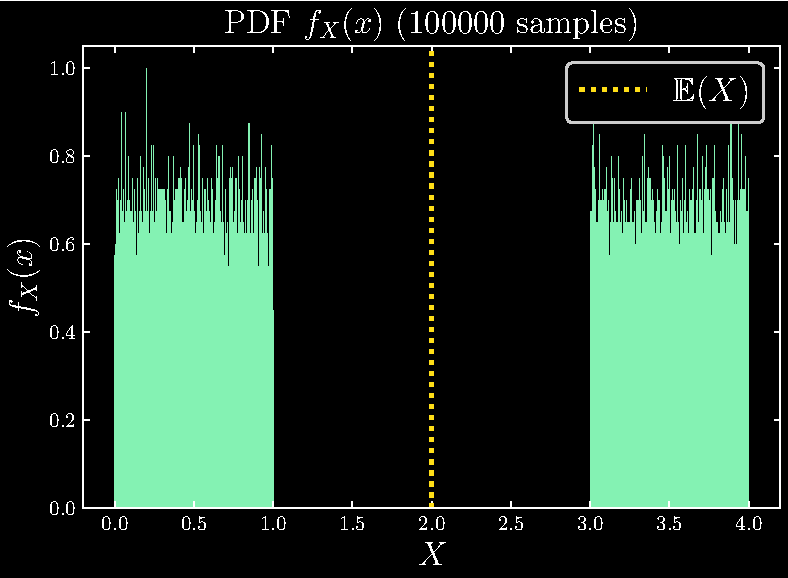
\includegraphics[width=1.0\textwidth]{chap3/chap3ex13.eps}
\end{center}

% QUESTION 14
\qs{3.8.14}{Let \(X_{1},\dots, X_{m}\) and \(Y_{1}, \dots, Y_{n}\) be random variables and let \(a_{1},\dots, a_{m}\) and \(b_{1},\dots, b_{n}\) be constants. Show that
\[
	\cov \left( \sum_{i=1}^{m} a_{i} X_{i}, \sum_{j=1}^{n} b_{j} Y_{j} \right) = \sum_{i=1}^{m} \sum_{j=1}^{n} a_{i} b_{j} \cov(X_{i}, Y_{j}).
\]}
\begin{proof}[Proof] 
By definition of \(\cov(X,Y)\):
\[
	\cov(X,Y) = \E \left((X - \mu_{X})(Y - \mu_{Y}) \right) 
\]
First, we will calculate the means of the two sums.
\begin{align*}
	\E \left( \sum_{i=1}^{m} a_{i} X_{i} \right)  & = \sum_{i=1}^{m} a_{i} \E(X_{i}) = \sum_{i=1}^{m} a_{i} \mu_{X_{i}} \\
	\E \left( \sum_{j=1}^{n} b_{j} Y_{j} \right)  & = \sum_{j=1}^{n} b_{j} \E(Y_{j}) = \sum_{j=1}^{n} b_{j} \mu_{Y_{j}} \\ 
\end{align*}
Proceeding from the definition of covariance, we can continue to derive
\[
	\cov \left( \sum_{i=1}^{m} a_{i} X_{i}, \sum_{j=1}^{n} b_{j} Y_{j} \right) 
\]
\begin{align*}
	 & = \E \left( \left( \sum_{i=1}^{m} a_{i}X_{i} - \sum_{i=1}^{m} a_{i}\mu_{X_{i}} \right) \left( \sum_{j=1}^{n} b_{j}Y_{j} - \sum_{j=1}^{n} b_{j} \mu_{Y_{j}} \right)  \right)  \\
	 & = \E \left( \left( \sum_{i=1}^{m} a_{i} (X_{i} - \mu_{X_{i}}) \right) \left( \sum_{j=1}^{n} b_{j}(Y_{j} - \mu_{Y_{j}} \right)  \right)  \\ 
	 & = \E \left( a_{1}(X_{1} - \mu_{X_{1}}) \sum_{j=1}^{n} b_{j}(Y_{j} - \mu_{Y_{j}}) + \cdots + a_{n}(X_{n} - \mu_{X_{n}}) \sum_{j=1}^{n} b_{j} (Y_{j}-\mu_{Y_{j}}) \right) \\
	 & = \E(a_{1}(X_{1} - \mu_{X_{1}})b_{1}(Y_{1} - \mu_{Y_{1}}) + \cdots + a_{1}(X_{1} - \mu_{X_{1}}) b_{n}(Y_{n} - \mu_{Y_{n}}) + \cdots\\
	 & \qquad + a_{n}(X_{1} - \mu_{X_{1}}) b_{1}(Y_{1} - \mu_{Y_{1}}) + \cdots + a_{n} (X_{1} - \mu_{X_{1}}) b_{n}(Y_{n} - \mu_{Y_{n}})) \\
	 & = \sum_{i=1}^{m} \sum_{j=1}^{n} \E(a_{i}b_{j}(X_{i} - \mu_{X_{i}})(Y_{j} - \mu_{Y_{j}})) \\
	 & = \sum_{i=1}^{m} \sum_{j=1}^{n} a_{i}b_{j} \cov(X_{i},Y_{j})
\end{align*}
\end{proof}

% QUESTION 15
\qs{3.8.15}{Let
\[
	f_{X,Y}(x,y) = \begin{cases}
		\frac{1}{3}(x+y) & 0 \le x \le 1, 0 \le y \le 2 \\
		0 & \text{otherwise.} \\
	\end{cases}	
\]
Find \(\var(2X-EY+8)\).}
The two approaches to this problem are to either use the definition \(\var(X) = \E(X^{2}) - \E(X)^{2}\), or to derive the marginal densities and individually calculate the expectations and variances for \(X,Y\). The first is far shorter, but we will solve using both methods.

Given \(\var(2X - 3Y + 8)\), observe that this is equivalent to \(\var(2X - 3Y)\), using the fact that constant terms do not affect the variance of a sum of random variables. Therefore we calculate
\[
	\var(2X - 3Y) = \E((2X-3Y)^{2}) - \E(2X-3Y)^{2}
\]
\begin{align*}
	\E((2X-3Y)^{2}) & = \int^{2}_{0} \int^{1}_{0} (2x-3y)^{2} \frac{1}{3} (x+y) \ dx  \ dy = \frac{86}{9}  \\
	\E(2X-3Y) & = \int^{2}_{0} \int^{1}_{0} (2x-3y) \frac{1}{3}(x + y) \ dx  \ dy = -\frac{23}{9} \\ 
	\var(2X-3Y) & = \frac{86}{9} - \left( -\frac{23}{9} \right)^{2} \\
		    & = \boxed{\frac{245}{81}}
\end{align*}

For the second method, begin with deriving the marginal densities:
\begin{align*}
	f_{X}(x) & = \int^{2}_{0} \frac{1}{3}(x + y) \ dy = \frac{2}{3}(x+1), \quad 0 \le x \le 1 \\
	f_{Y}(y) & = \int^{1}_{0} \frac{1}{3}(x + y) \ dx = \frac{1}{3} \left( \frac{1}{2} + y \right), \quad 0 \le y \le 2  \\ 
\end{align*}
The constituent expectations for calculations down the line are
\begin{align*}
	\E(X) & = \int^{1}_{0} \frac{2}{3}(x^{2} + x) \ dx = \frac{5}{9}  \\
	\E(X^{2}) & = \int^{1}_{0} \frac{2}{3}(x^{3} + x^{2}) \ dx = \frac{7}{18} \\ 
	\E(Y) & = \int^{2}_{0} \frac{1}{3}\left( y^{2} + \frac{y}{2} \right)  \ dy = \frac{11}{9} \\
	\E(Y^{2}) & = \int^{2}_{0} \frac{1}{3} \left( y^{3} + \frac{y^{2}}{2} \right)  \ dy = \frac{16}{9} \\
	\E(XY) & = \int^{2}_{0} \int^{1}_{0} xy f_{X,Y}(x,y) \ dx  \ dy\\
	       & = \int^{2}_{0} \int^{1}_{0} \frac{1}{3} (x^{2}y + xy^{2} \ dx  \ dy = \frac{2}{3} \\ 
\end{align*}
For the last step, the desired variance is calculated as
\[
	\var(2X - 3Y + 8) = 4 \var(X) + 9 \var(Y) - 12 \cov(X,Y)
\]
and the remaining quantities are
\begin{align*}
	\var(X) & = \E(X^{2}) - \E(X)^{2} = \frac{7}{18} - \left( \frac{5}{9} \right)^{2} = \frac{13}{162} \\
	\var(Y) & = \E(Y^{2}) - \E(Y)^{2} = \frac{16}{9} - \left( \frac{11}{9} \right)^{2} = \frac{23}{81} \\ 
	\cov(X,Y) & = \E(XY) - \E(X)\E(Y) \\
		  & = \frac{2}{3} - \left( \frac{5}{9} \right) \left( \frac{11}{9} \right) = -\frac{1}{81}
\end{align*}
At last, we combine the quantities to get
\begin{align*}
	\var(2X - 3Y + 8) & = 4 \var(X) + 9 \var(Y) - 12 \cov(X,Y) \\
	 & = 4 \left( \frac{13}{162} \right) + 9 \left( \frac{23}{81} \right) - 12 \left( -\frac{1}{81} \right)  \\ 
	 & = \boxed{\frac{245}{81}}
\end{align*}

% QUESTION 16
\qs{3.8.16}{Let \(r(x)\) be a function of \(x\) and let \(s(y)\) be a function of \(y\). Show that
\[
	\E(r(X)s(Y)  \mid  X) = r(X) \E(s(Y) \mid X).
\]
Also, show that \(\E(r(X)  \mid  X) = r(X)\).}
\begin{proof}[Proof] 
By definition of conditional expectation,
\begin{align*}
	\E(r(X)s(Y)) & = \int r(x) s(y) f_{Y \mid X}(y \mid x)  \ dy  \\
	 & = r(X) \int s(y) f_{Y \mid X}(y \mid x)  \ dy  \\ 
	 & = r(X) \E(s(Y) \mid X)
\end{align*}
For the second result, use the definition of conditional density.
\begin{align*}
	\E(r(X)  \mid  X) & = \int r(X) f_{Y \mid X}(y \mid x)  \ dy  \\
	 & = r(X) \int f_{Y \mid X}(y \mid x)  \ dy  \\ 
	 & = r(X) \int \frac{f_{X,Y}(x,y)}{f_{X}(x)} \ dy \\
	 & = r(X) \frac{f_{X}(x)}{f_{X}(x)} \\
	 & = r(X)
\end{align*}
\end{proof}

% QUESTION 16
\qs{3.8.16}{Prove that
\[
	\var(Y) = \E \var(Y  \mid  X) + \var \E(Y  \mid  X).
\]
Hint: Let \(m = \E(Y)\) and let \(b(x) = \E(Y  \mid  X = x)\). Note that \(\E(b(X)) = \E \E(Y  \mid  X) = \E(Y) = m\). Bear in mind that \(b\) is a function of \(x\). Now write \(\var(Y) = \E(Y-m)^{2} = \E((Y-b(X)) + (b(X) - m))^{2}\). Expand the square and take the expectation. You then have to take the expectation of three terms. In each case, use the rule of the iterated expectation: \(\E(\text{stuff}) = \E(\E(\text{stuff} \mid X)).\) }
\begin{proof}[Proof] 
Here we prove the Law of Total Variance. Together with the Law of Total Expectation, we establish Adam (expectation) and Eve's (variance) laws. Following the hints, derive
\begin{align*}
	\var(Y) & = \E(Y-m)^{2} \\
	 & = \E((Y - b(x)) + (b(x) - m))^{2} \\ 
	 & = \E((Y - b(x))^{2} + 2(Y - b(x))(b(x) - m) + (b(x) - m)^{2}) \\
	 & = \underbrace{\E(Y - b(x))^{2}}_{I} + \underbrace{2 \E((Y - b(x)) (b(x) - m))}_{II} + \underbrace{\E(b(x) - m)^{2}}_{III}		
\end{align*}
Terms I and III are easier to evaluate, applying the Law of Total Expectation in both:
\begin{align*}
	\E(Y - b(x))^{2} & = \E \E((Y - b(x))^{2}  \mid  X) \\
	 & = \E \left( \int (y - b(x))^{2} f_{Y \mid X}(y \mid x)  \ dy  \right)  \\
	 & = \E \var(Y  \mid  X) \\
	\E(b(X) - m)^{2} & = \E(b(x) - \E(b(x)))^{2} \\
	 & = \E \E((b(x) - \E(b(x)))^{2}  \mid  X) \\
	 & = \E \left( \int (b(x) - \E(b(x)))^{2} f_{Y \mid X}(y \mid x)  \ dy  \right) \\
	 & = \E \var(\E(Y \mid X)  \mid  X) \\
	 & = \var \E(Y  \mid  X)
\end{align*}

where \(b(x) = \E(Y  \mid  X) = \mu(x)\) in term I. To evaluate II, if we are to prove the desired result, we should end up with this term vanishing. Begin with
\begin{align*}
	\E((Y - b(x))(b(x) - m)) & = \E(Y \E(Y  \mid  X)) - \E(Y)^{2} \\
				 & \qquad - \E(\E(Y \mid X)^{2}) + \E(Y) \E(\E(Y \mid X)) \\
	 & = \E(Y \E(Y \mid X) - \E(Y \mid X)^{2}) - \E(Y)^{2} + \E(Y)^{2} \\ 
	 & = \E(\E(Y \mid X) (Y - \E(Y \mid X)))
\end{align*}
By the Law of Total Expectation, we can write as our next step
\[
	= \E(\E(\underbrace{\E(Y \mid X)}(Y - \E(Y \mid X)) \mid X))
\]
Now, using the results of exercise 3.8.16, we can pull the bracketed term out of the second nested expectation to get
\begin{align*}
	 & = \E(\E(Y \mid X) \E(Y - \E(Y \mid X)  \mid  X)) \\
	 & = \E(\E(Y \mid X) [\E(Y \mid X) - \E(\E(Y \mid X)  \mid  X)]) \\ 
	 & = \E(\E(Y \mid X)[\E(Y \mid X) - \E(Y \mid X)]) \\
	 & = 0
\end{align*}
Thereby proving
\begin{align*}
	\var(Y) = \E(Y-m)^{2} & = \E(Y - b(x))^{2} + \E(b(x) - m)^{2} \\
	 & = \E \var(Y \mid X) + \var \E(Y \mid X)  \\ 
\end{align*}

Note that this is a rather convoluted way to prove the Law of Total Variance; I am not sure why the author chose to gave the hints he did.
\end{proof}

% QUESTION 18
\qs{3.8.18}{Show that if \(\E(X  \mid  Y = y) = c\) for some constant \(c\), then \(X\) and \(Y\) are uncorrelated.}
\begin{proof}[Proof] 
Let \(\E(X  \mid  Y = y) = c\). Then the following are true:
\begin{enumerate}[label*=(\arabic*)]
	\item \(\E(\E(X  \mid  Y=y)) = \E(X) = \int x f_{X}(x) \ dx = \E(c) = c \)
	\item c = \( \int x f_{X \mid Y}(x \mid y)  \ dx = \int x \frac{f_{X,Y}(x,y)}{f_{Y}(y)} \ dx \)
\end{enumerate}
Combining these facts, we must have
\begin{alignat*}{3}
	&\implies &\int x f_{X}(x) \ dx & = \int x \frac{f_{X,Y}(x,y)}{f_{Y}(y)} \ dx \\
	&\implies &f_{X}(x) = \frac{f_{X,Y}(x,y)}{f_{Y}(y)} & \implies f_{X}(x) f_{Y}(y) = f_{X,Y}(x,y) \\ 
	& \implies & &X \sqcup Y \\
	& \implies & &\rho_{X,Y} = 0
\end{alignat*}
where the second implication follows from reasoning that
\[
	\int \left( x f_{X}(x) - x \frac{f_{X,Y}(x,y)}{f_{Y}(y)} \right) \ dx = \int x \left(f_{X}(x) - \frac{f_{X,Y}(x,y)}{f_{Y}(y)} \right) \ dx = 0
\]
But this equality holds only when the integrand is an odd function, or \(0\). Since we mandate no condition on the former, it must be the case that
\[
	f_{X}(x) = \frac{f_{X,Y}(x,y)}{f_{Y}(y)}
\]
\end{proof}

% QUESTION 19
\qs{3.8.19}{This question is to help you understand the idea of a \textbf{sampling distribution}. Let \(X_{1}, \dots, X_{n}\) be \textsf{IID} with mean \(\mu \) and variance \(\sigma^{2}\). Let \(\overline{X}_{n} = n^{-1} \sum_{i=1}^{n} X_{i}\). Then \(\overline{X}_{n}\) is a \textbf{statistic}, that is, a function of the data. Since \(\overline{X}_{n}\) is a random variable, it has a distribution. This distribution is called the \textit{sampling distribution of the statistic}. Recall from Theorem 3.17 that \(\E(\overline{X}_{n}) = \mu \) and \(\var(\overline{X}_{n}) = \sigma^{2}/n\). Don't confuse the distribution of the data \(f_{X}\left( x \right)\) and the distribution of the statistic \(f_{\bar{X}_{n}}\). To make this clear, let \(X_{1}, \dots, X_{n} \sim \Uniform(0,1)\). Let \(f_{X}\) be the density of the \(\Uniform(0,1)\). Plot \(f_{X}\). Now let \(\overline{X}_{n} = n^{-1} \sum_{i=1}^{n} X_{i}\). Find \(\E(\overline{X}_{n})\) and \(\var(\overline{X}_{n})\). Plot them as a function of \(n\). Interpret. Now simulate the distribution of \(\overline{X}_{n}\) for \(n = 1, 5, 25, 100\). Check that the simulated values of \(\E(\overline{X}_{n})\) and \(\var(\overline{X}_{n})\) agree with your theoretical calculations. What do you notice about the sampling distribution of \(\overline{X}_{n}\) as \(n\) increases?}

First, the density \(f_{X}\) of \(X \sim \Uniform\left( 0,1 \right)\) looks like

\begin{center}
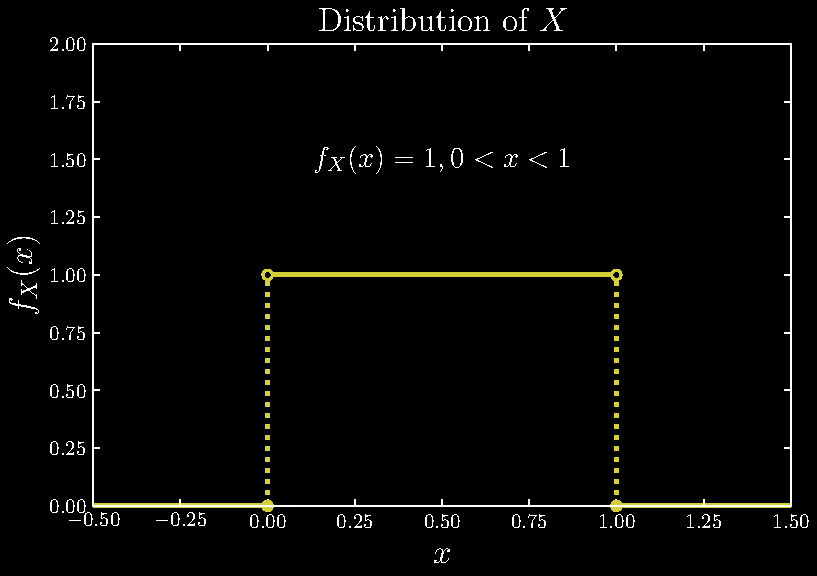
\includegraphics[width=1.0\textwidth]{chap3/chap3ex19i.eps}
\end{center}

Using the definition for \(\overline{X}_{n}\), the theoretical derivations of the expectation and variance are
\begin{align*}
	\E(\overline{X}_{n}) & = \frac{1}{n} \sum_{i=1}^{n} \E(X_{i}) \\
	 & = \frac{1}{n} \sum_{i=1}^{n} \int^{1}_{0} x_{i} \ dx_{i}  \\ 
	 & = \frac{1}{n} \sum_{i=1}^{n} \frac{1}{2} \\
	 & = \boxed{\frac{1}{2}} 
\end{align*}
Now, \(\overline{X}_{n}^{2}\) is given by
\begin{align*}
	\overline{X}_{n}^{2} & = \frac{1}{n^{2}} \left( \sum_{i=1}^{n} X_{i} \right)^{2} \\
			     & \frac{1}{n^{2}} \left( \underbrace{\sum_{i=1}^{n} X_{i}^{2}}_{n \text{ terms}} + \underbrace{\sum_{i=1}^{n} \sum_{\substack{j \neq i \\ j = 1} }^{n} X_{i} X_{j}}_{n(n-1) \text{ terms}} \right)  \\ 
\end{align*}
Using the fact that the random variables are \textsf{IID}, we can derive
\begin{align*}
	\E(\overline{X}_{n}^{2}) & = \frac{1}{n^{2}} \left( \sum_{i=1}^{n} \int^{1}_{0} x_{i}^{2} \ dx_{i} + \sum_{i=1}^{n} \sum_{\substack{j \neq i \\ j = 1}}^{n} \int^{1}_{0} x_{i} \ dx_{i} \int^{1}_{0} x_{j} \ dx_{j}    \right)  \\
	 & = \frac{1}{n^{2}} \left( n \left( \frac{1}{3} \right) + n(n-1) \left( \frac{1}{2} \right) \left( \frac{1}{2} \right)  \right)  \\ 
	 & = \frac{1}{n^{2}} \left( \frac{1}{4} n^{2} - \frac{1}{4}n + \frac{1}{3}n \right) \\
	 & = \frac{1}{4} + \frac{1}{12n} \\
	\var(\overline{X}_{n}) & = \E(\overline{X}_{n}^{2}) - \E(\overline{X}_{n})^{2} \\
	 & = \frac{1}{12n} + \frac{1}{4} - \left( \frac{1}{2} \right)^{2} \\
	 & = \boxed{\frac{1}{12n}}
\end{align*}

Empirically, we can verify that randomly generating a sampling distribution of values of \(\overline{X}_{n}\) and taking the expectation and variance agrees with the theory:

\begin{center}
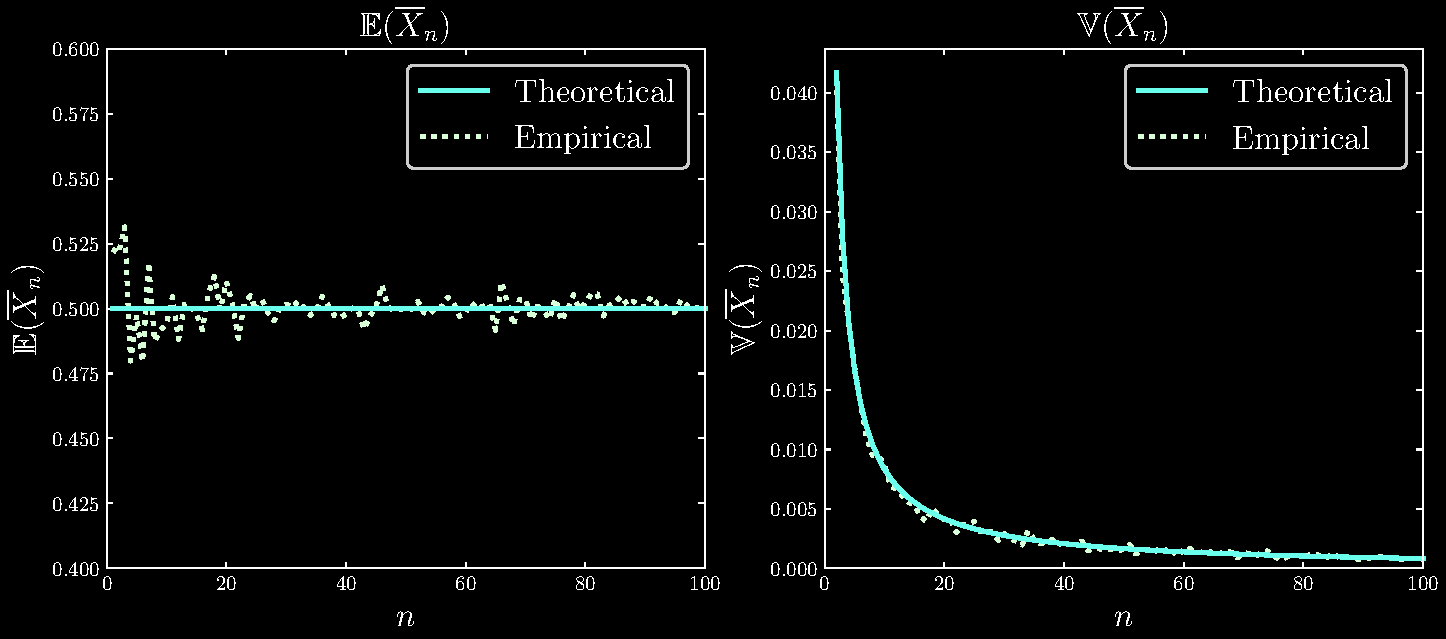
\includegraphics[width=1.0\textwidth]{chap3/chap3ex19ii.eps}
\end{center}

Lastly, we graph the sampling distributions as \(n\) increases:

\begin{center}
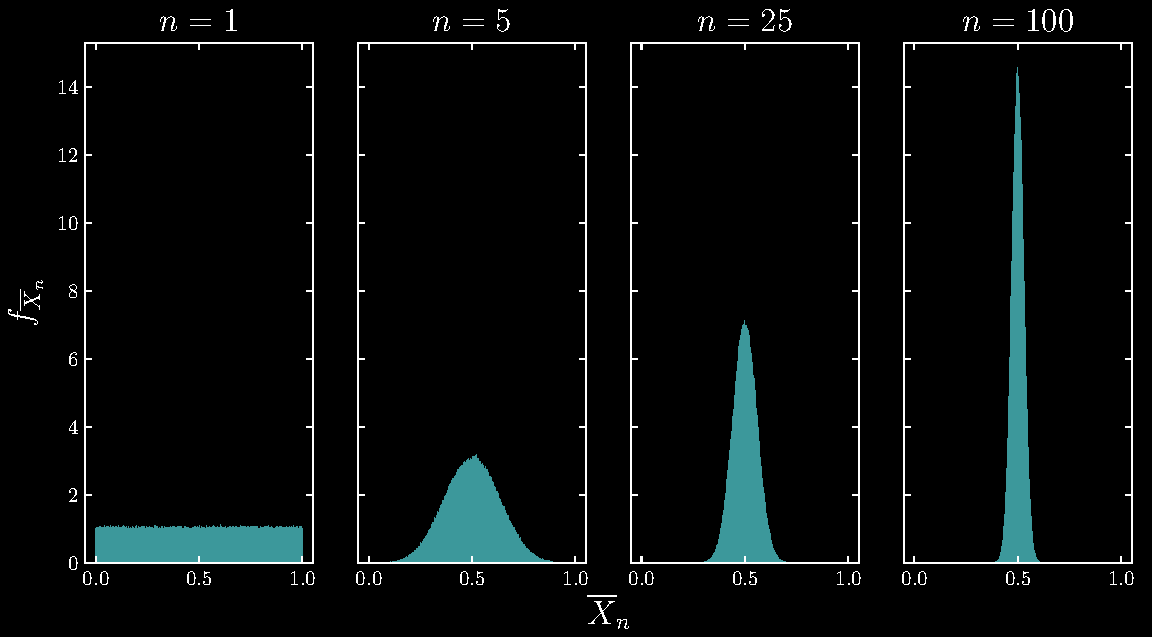
\includegraphics[width=1.0\textwidth]{chap3/chap3ex19iii.eps}
\end{center}

which gradually increases in concentration (\(\var\left( \overline{X}_{n} \right)\) goes to \(0\)) around the mean \(\E\left( \overline{X}_{n} \right) = 1/2\).

% QUESTION 20
\qs{3.8.20}{Prove Lemma 3.21.}
\lemma{(Wasserman 3.21)}{If \(a\) is a vector and \(X\) is a random vector with mean \(\mu \) and variance \(\Sigma\), then \(\E(a^{T} X) = a^{T} \mu\) and \(\var(a^{T}X) = a^{T} \Sigma a\). If \(A\) is a matrix then \(\E(AX) = A \mu \) and \(\var(AX) = A \Sigma A^{T}\). }
\begin{proof}[Proof] 
Let \(a, X \in M_{n \times 1}\), where \(M_{n \times 1}\) is the set of \(n \times 1\) vectors, and \(X\) is a random vector with mean \(\mu \) and variance \(\Sigma\).

By vector multiplication and the definition of a random vector mean, we first derive
\[
	\E(a^{T}X) = \E \left( \sum_{i=1}^{n} a_{i} X_{i} \right)  = \sum_{i=1}^{n} \E(X_{i}) = \sum_{i=1}^{n} a_{i} \mu_{i} = a^{T}\mu 
\]
Now using the definition of the variance-covariance matrix \(\Sigma\), we have \(\var(a^{T}X)\) equal to
\begin{align*}
	 & = \var \left( \sum_{i=1}^{n} a_{i} X_{i} \right)  \\
	 & = \sum_{i=1}^{n} a_{i}^{2} \var(X_{i}) + 2 \sum_{i=1}^{n} \sum_{i < j}^{n} a_{i} a_{j} \cov(X_{i}, X_{j}) \\ 
	 & = \begin{bmatrix}
		a_{1} & \cdots & a_{n} \\
	\end{bmatrix}
	 \begin{bmatrix}
		\var(X_{1}) & \cov(X_{1}, X_{2}) & \cdots & \cov(X_{1}, X_{n})  \\
		\cov(X_{2}, X_{1}) & \var(X_{2}) & \cdots & \cov(X_{2}, X_{n}) \\
		\vdots  & \vdots & \vdots & \vdots \\
		 \cov(X_{n}, X_{1}) & \cov(X_{n}, X_{2}) & \cdots & \var(X_{n}) \\
	\end{bmatrix}
	\begin{bmatrix}
		a_{1} \\
		\vdots \\
		a_{n} \\
	\end{bmatrix} \\
	 & = a^{T} \Sigma a
\end{align*}
Now let \(A \in M_{n \times n}\). Then
\[
	AX = 
	\begin{bmatrix}
		a_{11} & \cdots  & a_{1n} \\
		a_{21} & \cdots  & a_{2n} \\
		\vdots & \ddots & \vdots \\
		a_{n1} & \cdots & a_{nn}
	\end{bmatrix}
	\begin{bmatrix}
	        X_{1} \\
		X_{2} \\
		\vdots \\
		X_{n} \\
	\end{bmatrix}
	=
	\begin{bmatrix}
		\sum_{i=1}^{n} a_{1i} X_{i} \\
		\vdots \\
		\sum_{i=1}^{n} a_{ni} X_{i} \\
	\end{bmatrix}
\]
which has expectation
\begin{align*}
	\E(AX) & =
	\E\begin{bmatrix}
		\sum_{i=1}^{n} a_{1i} X_{i} \\
		\vdots \\
		\sum_{i=1}^{n} a_{ni} X_{i} \\
	\end{bmatrix} \\
	       & =
	\begin{bmatrix}
		\sum_{i=1}^{n} a_{1i} \E(X_{i}) \\
		\vdots \\
		\sum_{i=1}^{n} a_{ni} \E(X_{i}) \\
	\end{bmatrix} \\
	       & =
	\begin{bmatrix}
		\sum_{i=1}^{n} a_{1i} \mu_{i} \\
		\vdots \\
		\sum_{i=1}^{n} a_{ni} \mu_{i} \\
	\end{bmatrix} \\
	       & =
	\begin{bmatrix}
		a_{11} & \cdots  & a_{1n} \\
		a_{21} & \cdots  & a_{2n} \\
		\vdots & \ddots & \vdots \\
		a_{n1} & \cdots & a_{nn} \\
	\end{bmatrix}
	\begin{bmatrix}
		\mu_{1} \\
		\mu_{2} \\
		\vdots \\
		\mu_{n} \\
	\end{bmatrix} \\
	 & = A \mu \\ 
\end{align*}
and variance \(\var(AX)\) equal to
\[
	\begingroup
	\setlength\arraycolsep{2pt}
	\begin{bmatrix}
		\var ( \sum a_{1i} X_{i} )  & \cov(\sum a_{1i} X_{i}) &\cdots & \cov(\sum a_{1i} X_{i}, \sum a_{ni} X_{i})  \\
		\cov(\sum a_{2i} X_{i}, \sum a_{1i} X_{i}) & \var(\sum a_{2i} X_{i}) & \cdots & \cov(\sum a_{2i} X_{i}, \sum a_{ni} X_{i}) \\
		\vdots & \vdots & \vdots & \vdots \\
		\cov(\sum a_{ni} X_{i}, \sum a_{1i} X_{i}) & \cov(\sum a_{ni} X_{i}, \sum a_{2i} X_{i}) & \cdots & \var(\sum a_{ni} X_{i}) \\
	\end{bmatrix}
	\endgroup
\]
To further simplify, use the result of exercise 14 to get
\[
	\begin{bmatrix}
		\substack{\sum\limits_{i=1}^{n} a_{1i}^{2} \var(X_{i}) \\ + 2 \sum\limits_{i=1}^{n-1} \sum\limits_{i < j}^{n} a_{1i} a_{1j} \cov(X_{i}, X_{j})} & \cdots  & \sum\limits_{i=1}^{n} \sum\limits_{j=1}^{n} a_{1i} a_{1j} \cov(X_{i}, X_{j}) \\
		\sum\limits_{i=1}^{n} \sum\limits_{j=1}^{n} a_{2i} a_{1j} \cov(X_{i}, X_{j}) & \cdots  & \sum\limits_{i=1}^{n} \sum\limits_{j=1}^{n} a_{2i} a_{nj} \cov(X_{i}, X_{j}) \\
		\vdots & \ddots & \vdots \\
		\sum\limits_{i=1}^{n} \sum\limits_{j=1}^{n} a_{ni} a_{1j} \cov(X_{i}, X_{j}) & \cdots & \substack{\sum\limits_{i=1}^{n} a_{ni}^{2} \var(X_{i}) \\ + 2 \sum\limits_{i=1}^{n-1} \sum\limits_{i < j}^{n} a_{ni} a_{nj} \cov(X_{i}, X_{j})}
	\end{bmatrix}
\]
for which each entry is precisely the value of each entry in the matrix product
\[
	\begingroup
	\setlength\arraycolsep{1.55pt}
	\begin{bmatrix}
		a_{11} & \cdots  & a_{1n} \\
		a_{21} & \cdots  & a_{2n} \\
		\vdots & \ddots & \vdots \\
		a_{n1} & \cdots  & a_{nn} \\
	\end{bmatrix}
	\begin{bmatrix}
		\var(X_{1}) & \cov(X_{1}, X_{2}) & \cdots  & \cov(X_{1}, X_{n}) \\
		\cov(X_{2}, X_{1}) & \var(X_{2}) & \cdots & \cov(X_{2}, X_{n}) \\
		\vdots & \vdots & \vdots & \vdots \\
		\cov(X_{n}, X_{1}) & \cov(X_{n},X_{2}) & \cdots  & \var(X_{n}) \\
	\end{bmatrix}
	\begin{bmatrix}
		a_{11} & a_{21} & \cdots  & a_{n1} \\
		\vdots & \vdots & \ddots & \vdots \\
		a_{1n} & a_{2n} & \cdots  & a_{nn} \\
	\end{bmatrix}
	\endgroup
\]
which is \(\var(AX) = A \Sigma A^{T}\), as desired.
\end{proof}

% QUESTION 21
\qs{3.8.21}{Let \(X\) and \(Y\) be random variables. Suppose that \(\E(Y \mid X) = X\). Show that \(\cov(X,Y) = \var(X)\).}
\begin{proof}[Proof] 
Let \(\E(Y  \mid  X) = X\). Then \(\E(\E(Y  \mid  X)) = \E(Y) = \E(X)\). Moreover,
\[
	x = \int y f_{Y \mid X}(y \mid x) \ dy = \int y \frac{f_{Y,X}(y,x)}{f_{X}(x)} \ dy
\]
This implies
\begin{alignat*}{3}
	&\implies & x^{2} f_{X}(x) & = \int xy f_{Y,X}(y,x) \ dy \\
	&\implies & \int x^{2} f_{X}(x) \ dx & = \int \int xy f_{Y,X}(y,x) \ dy \ dx \\ 
	&\implies & \E(X^{2}) & = \E(XY) \\
	&\implies & \cov(X,Y) & = \E(XY) - \E(X) \E(Y) \\
	& & & = \E(X^{2}) - \E(X)^{2} \\
	& & & = \var(X)
\end{alignat*}
\end{proof}

% QUESTION 22
\qs{3.8.22}{Let \(X \sim \Uniform(0,1)\). Let \(0 < a < b < 1\). Let
\[
	Y = \begin{cases}
		1 & 0 < x < b \\
		0 & \text{otherwise} \\
	\end{cases}
\]
and let
\[
	Z = \begin{cases}
		1 & a < x < 1 \\
		0 & \text{otherwise} \\
	\end{cases}
\]
\begin{enumerate}[label=(\alph*)]
	\item Are \(Y\) and \(Z\) independent? Why/Why not?
	\item Find \(\E(Y \mid Z)\). Hint: What values \(z\) can \(Z\) take? Now find \(\E(Y  \mid  Z = z)\).
\end{enumerate}}

(a) The probabilities for all values of \(Y,Z\) are
\begin{align*}
	\Prob(Y=1) & = \int^{b}_{0}  \ dx  = b \\
	\Prob(Y=0) & = \int^{1}_{b}  \ dx = 1-b  \\ 
	\Prob(Z=1) & = \int^{1}_{a}  \ dx = 1-a \\
	\Prob(Z=0) & = \int^{a}_{0}  \ dx = a 
\end{align*}
Now, consider the following case
\[
	\Prob(Y=1,Z=1) = \int^{b}_{a}  \ dx = b-a 
\]
However,
\[
	\Prob(Y=1)\Prob(Z=1) = b(1-a) != b-a = \Prob(Y=1,Z=1)
\]
Thus \(Y\) and \(Z\) are not independent.

\par (b) The conditional expectations are
\[
	\E(Y  \mid  Z) = \begin{cases}
		\begin{aligned}
		& 1 \cdot \Prob(Y  \mid  Z=0) = \frac{\int^{a}_{0}  \ dx }{\int^{a}_{0}  \ dx } = 1 & \quad z = 0 \\
		& 1 \cdot \Prob(Y  \mid  Z=1) = \frac{\int^{b}_{a}  \ dx }{\int^{1}_{a}  \ dx } = \frac{b-a}{1-a} & \quad z = 1 \\
	\end{aligned}
	\end{cases}
\]
\newpage
% QUESTION 23
\qs{3.8.23}{Find the moment generating function for the Poisson, Normal, and Gamma distributions.}
\underline{Poisson}

For \(X \sim \Poisson(\lambda )\), we have mass
\[
	f_{X}(x) = e^{-\lambda } \frac{\lambda^{x}}{x!}
\]
with moment generating function
\begin{align*}
	\psi_{X}(t) & = \sum_{x-0}^{\infty} e^{tx} e^{-\lambda } \frac{\lambda^{x}}{x!} \\
	 & = e^{-\lambda } \sum_{x=0}^{\infty} \frac{(\lambda e^{t})^{x}}{x!} \\ 
	 & = e^{-\lambda } e^{\lambda e^{t}} \\
	 & = \boxed{e^{\lambda (e^{t} - 1)}}
\end{align*}

\underline{Normal}

For \(X \sim N(0,1)\), we have density
\[
	f_{X}(x) = \frac{1}{\sigma \sqrt{2 \pi }} \exp \left( -\frac{1}{2 \sigma^{2}} (x-\mu)^{2} \right) 
\]
with moment generating function
\begin{align*}
	\psi_{X}(t) = \E(e^{tx}) & = \frac{1}{\sigma \sqrt{2 \pi }} \int \exp \left( -\frac{1}{2 \sigma^{2}}(x-\mu)^{2} + tx \right) \ dx \\
	 & = \frac{1}{\sigma \sqrt{2 \pi }} \int \exp \left( -\frac{1}{2 \sigma^{2}} (x^{2} - 2 \mu x + \mu^{2}) + tx \right) \ dx \\ 
	 & = \frac{1}{\sigma \sqrt{2 \pi }} \int \exp \left( -\frac{1}{2 \sigma^{2}} x^{2} + \left( \frac{\mu }{\sigma^{2}} + t \right)x - \frac{\mu^{2}}{2 \sigma^{2}} \right) \ dx \\
	 & = \frac{1}{\sigma \sqrt{2 \pi }} \exp \left( -\frac{\mu^{2}}{2 \sigma^{2}} \right) \int \exp \left( -\frac{1}{2 \sigma^{2}}x^{2} + \left( \frac{\mu }{\sigma^{2}} + t \right) x \right)   \ dx 
\end{align*}
Here we complete the square by adding and subtracting \((\sigma^{2}/2)(\mu/\sigma^{2} + t)^{2}\), and writing
\[
	= \frac{1}{\sigma \sqrt{2 \pi }} \int \exp \left( -\frac{\mu^{2}}{2 \sigma^{2}} ( x - (\mu + \sigma^{2} t))^{2} + \frac{\sigma^{2}}{2} \left( \frac{\mu }{\sigma^{2}} + t \right)^{2} \right) \ dx
\]
Now substitute \(u = x - (\mu + \sigma^{2}t)\). Then \(du = dx\), and
\begin{align*}
	 & = \frac{1}{\sigma \sqrt{2 \pi }} \exp \left( -\frac{\mu^{2}}{2 \sigma^{2}} + \frac{\sigma^{2}}{2} \left( \frac{\mu }{\sigma^{2}} + t \right)^{2} \right) \int \exp \left( -\frac{1}{2 \sigma^{2}} \mu^{2} \right) \ du \\
	 & = \exp \left( -\frac{\mu^{2}}{2 \sigma^{2}} + \frac{\sigma^{2}}{2} \left( \frac{\mu }{\sigma^{2}} + t \right)^{2} \right)  \\ 
	 & = \exp \left( -\frac{\mu^{2}}{2 \sigma^{2}} + \frac{\sigma^{2}}{2} \left( \frac{\mu^{2}}{\sigma^{4}} + \frac{2 \mu }{\sigma^{2}} t + t^{2} \right)  \right) \\
	 &= \boxed{\exp \left( \mu t + \frac{1}{2} \sigma^{2} t^{2} \right) }
\end{align*}

\underline{Gamma }

For \(X \sim \gammaD(\alpha ,\beta )\), we have density
\[
	f_{X}(x) = \frac{1}{\beta^{\alpha } \Gamma(\alpha )} x^{\alpha -1} e^{-x/\beta }, \quad x, \alpha, \beta > 0
\]
where
\[
	\Gamma(\alpha ) = \int^{\infty}_{0} y^{\alpha -1} e^{-y} \ dy 
\]
and with moment generating function
\[
	\psi_{X}(t) = \E(e^{tx}) = \frac{1}{\beta^{\alpha } \Gamma(\alpha )} \int^{\infty}_{0} x^{\alpha -1} e^{-x(1/\beta - t)} \ dx 
\]
Let \(y = x (1/\beta -t)\). Then \(dy = (1/\beta -t)dx\), and we have for \(t < 1/\beta \)
\begin{align*}
	 & = \frac{1}{\beta^{\alpha } \Gamma(\alpha )} \frac{1}{(1/\beta - t)^{\alpha }} \int^{\infty}_{0} y^{\alpha -1} e^{-y} \ dy  \\
	 & = \frac{1}{\beta^{\alpha } \Gamma(\alpha )} \frac{1}{(1/\beta^{\alpha }) (1-t \beta )^{\alpha }}\Gamma(\alpha ) \\ 
	 & = \boxed{(1 - t \beta )^{-\alpha }}
\end{align*}

% QUESTION 24
\qs{3.8.24}{Let \(X_{1}, dots, X_{n} \sim \Exp(\beta )\). Find the moment generating function of \(X_{i}\). Prove that \(\sum_{i=1}^{n} X_{i} \sim \gammaD(n, \beta )\).}
\begin{proof}[Proof] 
For \(X_{i} \sim \Exp(\beta )\), we have density
\[
	f_{X_{i}}(x_{i}) = \frac{1}{\beta } \exp(-x_{i}/\beta ), \quad x_{i}, \beta >0
\]
with moment generating function
\begin{align*}
	\psi_{X_{i}}(t) = \E(e^{tx}) & = \frac{1}{\beta } \int^{\infty}_{0} \exp(-x(1/\beta -t) \ dx  \\
	 & = \frac{1}{1-t \beta } 
\end{align*}
for \( t < 1/\beta \). By Lemma 3.31(2) and assuming independence of the \(X_{i}\)'s, for \(X = \sum_{i=1}^{n} X_{i}\) we have
\[
	\psi_{X}(t) = \prod_{i} \psi_{X_{i}}(t) = \prod_{i} (1 - t \beta ) = (1-t \beta )^{-n}   
\]
Implying \(X \sim \gammaD(n, \beta )\) per the results of exercise 3.8.23.

\end{proof}

\end{document}
